% Author: Taejin Hwang, Paul Shao

\learning{
Understand how to apply properties of inner products, cross correlations, trilateration, least squares, and OMP to build an acoustic positioning system. Learn how to identify the pros/cons when applying different techniques in building the system.}
\\ \\
In this question, we will revisit the \textbf{Acoustic Positioning System} (APS) and learn how to build it from the ground up using what we know about cross correlation, trilateration, least squares, and Orthogonal Matching Pursuit (OMP).
\\ \\
Recall that in an APS, we have a number of satellites (let's say there are $m$) transmitting gold codes, and you are a person standing at a location with the coordinate $\vec{x}$, with your phone as the receiver of the signals.
\\ \\
You receive a linear combination of these transmitted signals, each delayed by $(\tau_i)$:
$$\vec{r} = \alpha_1 \vec{s}_1^{\ (\tau_1)} + \alpha_2 \vec{s}_2^{\ (\tau_2)} + \hdots + \alpha_m \vec{s}_m^{\ (\tau_m)}$$
As shown in the expression above, each signal is scaled by a constant which is a \textit{"message"} the satellite encodes into its signal while transmitting.
\\ \\
To solve for our current position, we can set up a system of equations based on our current position $\vec{x}$, the position of each satellite $\vec{p}_1, \vec{p}_2, \hdots, \vec{p}_m$, and the distance from our current position to each satellite $d_i$.
\\ \\
Here's an illustration of the APS (given 3 satellites):
\begin{figure}[H]
    \centering
    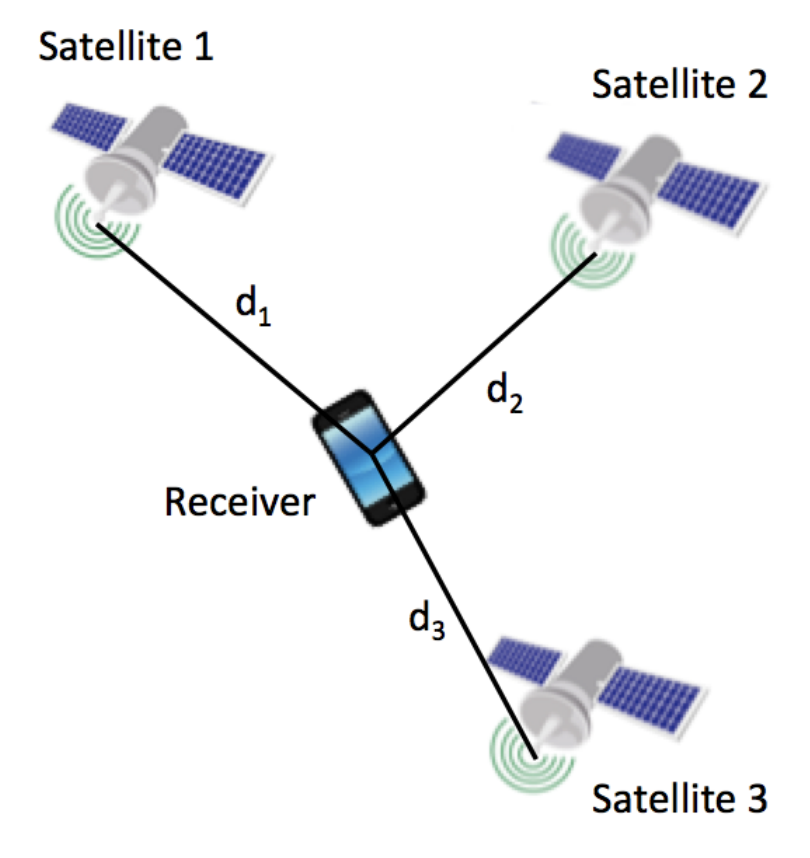
\includegraphics[scale=0.45]{../trilateration-1}
\end{figure}

\begin{enumerate}
    \item Based on the provided information above, which of the following variables are known? Which are unknown (the ones we are trying to solve for)?

        \begin{itemize}
            \item The position of each satellite $\vec{p}_i$
            \item Our current position $\vec{x}$
            \item The transmitted signals $\vec{s}_i^{\ (\tau_i)}$
            \item The distances from our current position to each satellite $d_i$
            % \item The time delay of each signal $\tau_1, \ldots, \tau_m$
            % \item The messages $\alpha_1, \ldots, \alpha_m$
        \end{itemize}
    \answerbox{2cm}

    \sol {
      \begin{itemize}
            \item The position of each satellite $\vec{p}_i:$
            These are \textbf{known} variables since we as the engineer have placed these satellites out in space.
            \item Our current position $\vec{x}:$
            This is an $\textbf{unknown}$ variable that we are trying to determine using the satellites and received signal.
            \item The transmitted signals $\vec{s}_i^{\ (\tau_i)}:$
            These are \textbf{known} variables that we as the engineer have programmed, hopefully using Gold Codes.
            \item The distances from our current position to each satellite $d_i:$
            These an $\textbf{unknown}$ variables since we don't know our current position $\vec{x}.$
            % \item The time delay of each signal $\tau_1, \ldots, \tau_m.$
            % These are \textbf{unknown} variables as well, since we don't know the distance from our current position to the satellites. Note that $d_i$ and $\tau_i$ are related by the physics equation $d = v \cdot t$ where $v$ is the speed of light and $t$ is the time delay in seconds.
            % \item The messages $\alpha_1, \ldots, \alpha_m:$ 
            % These are \textbf{unknown} variables that we need to solve for since we receive one signal $\vec{r}$ that is a linear combination of the satellite signals and $\alpha_i$ are the weights of this linear combination.
      \end{itemize}
    }

    \item We will start by solving for the distances $d_{i}$ and the time delays $\tau_{i}.$ How can we compute these quantities using the received signal $\vec{r}$ and the Gold-Codes for each satellite, $\vec{s}_{i}?$

    \note {
        Note that $\tau_{i}$ is an integer which represents the time shift for the discrete signal $\vec{s}_{i}.$
        Therefore to compute the distance $d_{i}$ in meters, the time delay $\tau_{i}$ must be converted into seconds.
        This is out of scope, but can be done based on the sampling rate of the receiver, and should only be addressed if students ask about it.
    }

    \sol {
        We can solve for the time delay $\tau_{i}$ by computing the cross-correlation between $\vec{r}$ and $\vec{s}_{i}.$
        \[ \text{corr}_{\vec{r}}(\vec{s}_{i})[k] = \sum\limits_{n = -\infty}^{\infty} \vec{r}[n] \vec{s}_{i}[n - k] \]
        Remember that the cross-correlation between two vectors $\vec{r}, \vec{s}_{i}$ measures the similarity between $\vec{r}$ with all shifts of $\vec{s}_{i}.$
        Therefore, we pick the index $\tau_{i}$ as the index of greatest cross-correlation between $\vec{r}$ and $\vec{s}_{i}.$
        The distance $d_{i}$ can be computed by multiplying the time delay by the speed of light.
    }

    \item How can we express $d_i$ in terms of $\vec{p}_i$ and $\vec{x}$? How many such equations can we set up in total?

    \answerbox{5cm}

    \note {
        Mentors, it might be helpful to draw out or point to the APS illustration to show why it is natural to label distances as the norms of the differences in position.
    }

    \sol {
        It can be observed that the norm of the difference between $\vec{x}$ and $\vec{p}_{i}$ will indeed be the distance $d_{i}$ from $\vec{x}$ to $\vec{p}_{i}.$
        Therefore for each satellite, we can write out the equations:
        \begin{align*}
            \norm{\vec{x} - \vec{p}_{1}} &= d_{1} \\
            &\vdots \\
            \norm{\vec{x} - \vec{p}_{m}} &= d_{m} 
        \end{align*}
        There will be a total of $m$ equations since we get one equation for each satellite.
    }

    \item Recall that an APS can help us determine where we are. Which variable given in the question corresponds to our current location? Also, based on the system of equations we set up in part 3, how can we solve for our current position?

    \answerbox{7cm}

    \sol {
        The vector $\vec{x}$ corresponds to our current location. As seen in the first and second parts, we know the location of each satellite $\vec{p}_{i}$ and we have also solved for the distances $d_{i}.$ Therefore it remains to solve the system of equations we created in the previous part. 

        We will first take a look at satellite $1$ and then generalize for the rest. First we can square both sides and expand out the norms:
        \begin{align*}
        \norm{\vec{x} - \vec{p}_{1}}^{2} &= \innp{\vec{x} - \vec{p}_{1}, \vec{x} - \vec{p}_{1}} = (\vec{x} - \vec{p}_{1})^{T}(\vec{x} - \vec{p}_{1}) \\
        &= \vec{x}^{T} \vec{x} - \vec{p}_{1}^{T} \vec{x} - \vec{x}^{T} \vec{p}_{1} + \vec{p}_{1}^{T} \vec{p}_{1} = \vec{x}^{T} \vec{x} - 2 \vec{p}_{1}^{T} \vec{x} + \vec{p}_{1}^{T} \vec{p}_{1} = d_{1}^{2}
        \end{align*}
        We can then do this for any satellite $i$ to say that
        \begin{align*}
            \norm{\vec{x} - \vec{p}_{1}}^{2} &= \vec{x}^{T} \vec{x} - 2 \vec{p}_{1}^{T} \vec{x} + d_{1}^{2} \\
            &\vdots \\
            \norm{\vec{x} - \vec{p}_{m}} &= \vec{x}^{T} \vec{x} - 2 \vec{p}_{m}^{T} \vec{x} + d_{m}^{2} 
        \end{align*}
        While we have a system of equations that we could try solving, the issue is the quadratic term $\vec{x}^{T} \vec{x}.$ 
        Therefore, we will get rid of this quadratic term by subtracting every equation from the first equation to get
        \begin{align*}
            2 \vec{p}_{1}^{T} \vec{x} - 2 \vec{p}_{2}^{T} \vec{x} &= d_{2}^{2} - d_{1}^{2} \\
            &\vdots \\
            2 \vec{p}_{1}^{T} \vec{x} - 2 \vec{p}_{m}^{T} \vec{x} &= d_{m}^{2} - d_{1}^{2}
        \end{align*}
        We can now set up the following matrix-vector equation:
        \[
            \begin{bmatrix} 
            2 (\vec{p}_{1}^{T} - \vec{p}_{2}^{T}) \\
            \vdots \\
            2 (\vec{p}_{1}^{T} \vec{x} - \vec{p}_{m}^{T})
            \end{bmatrix} \vec{x} = 
            \begin{bmatrix} 
            d_{2}^{2} - d_{1}^{2} \\
            \vdots \\
            d_{m}^{2} - d_{1}^{2}
            \end{bmatrix}
        \]
        $\vec{x}$ can be solved either through Gaussian-Elimination, Inversion, or Least Squares depending on the shape of the matrix.
    }

    \item If our current position can be represented by an $n$-dimensional vector, how many satellites do we need to be able to solve for our position?

    \sol {
        If the position $\vec{x}$ is an $n$-dimensional vector, the system of equations will have $n$ unknowns.
        This means we need $n$ linear equations to solve this system uniquely. 
        Each satellite will bring in one equation, but remember that these were nonlinear, meaning we had to subtract an equation out to get rid of the quadratic term. Therefore we will need $n + 1$ equations total, or $n + 1$ satellite measurements.
    }
    \answerbox{1cm}

    \item As shown below geometrically, we can represent the area of coverage by each satellite as a circle with a radius of $d_i$. Explain why the radius of each circle is $d_i$, and how finding our current position is equivalent to finding the point of intersection among the circumferences of the circles.
    \begin{figure}[H]
        \centering
        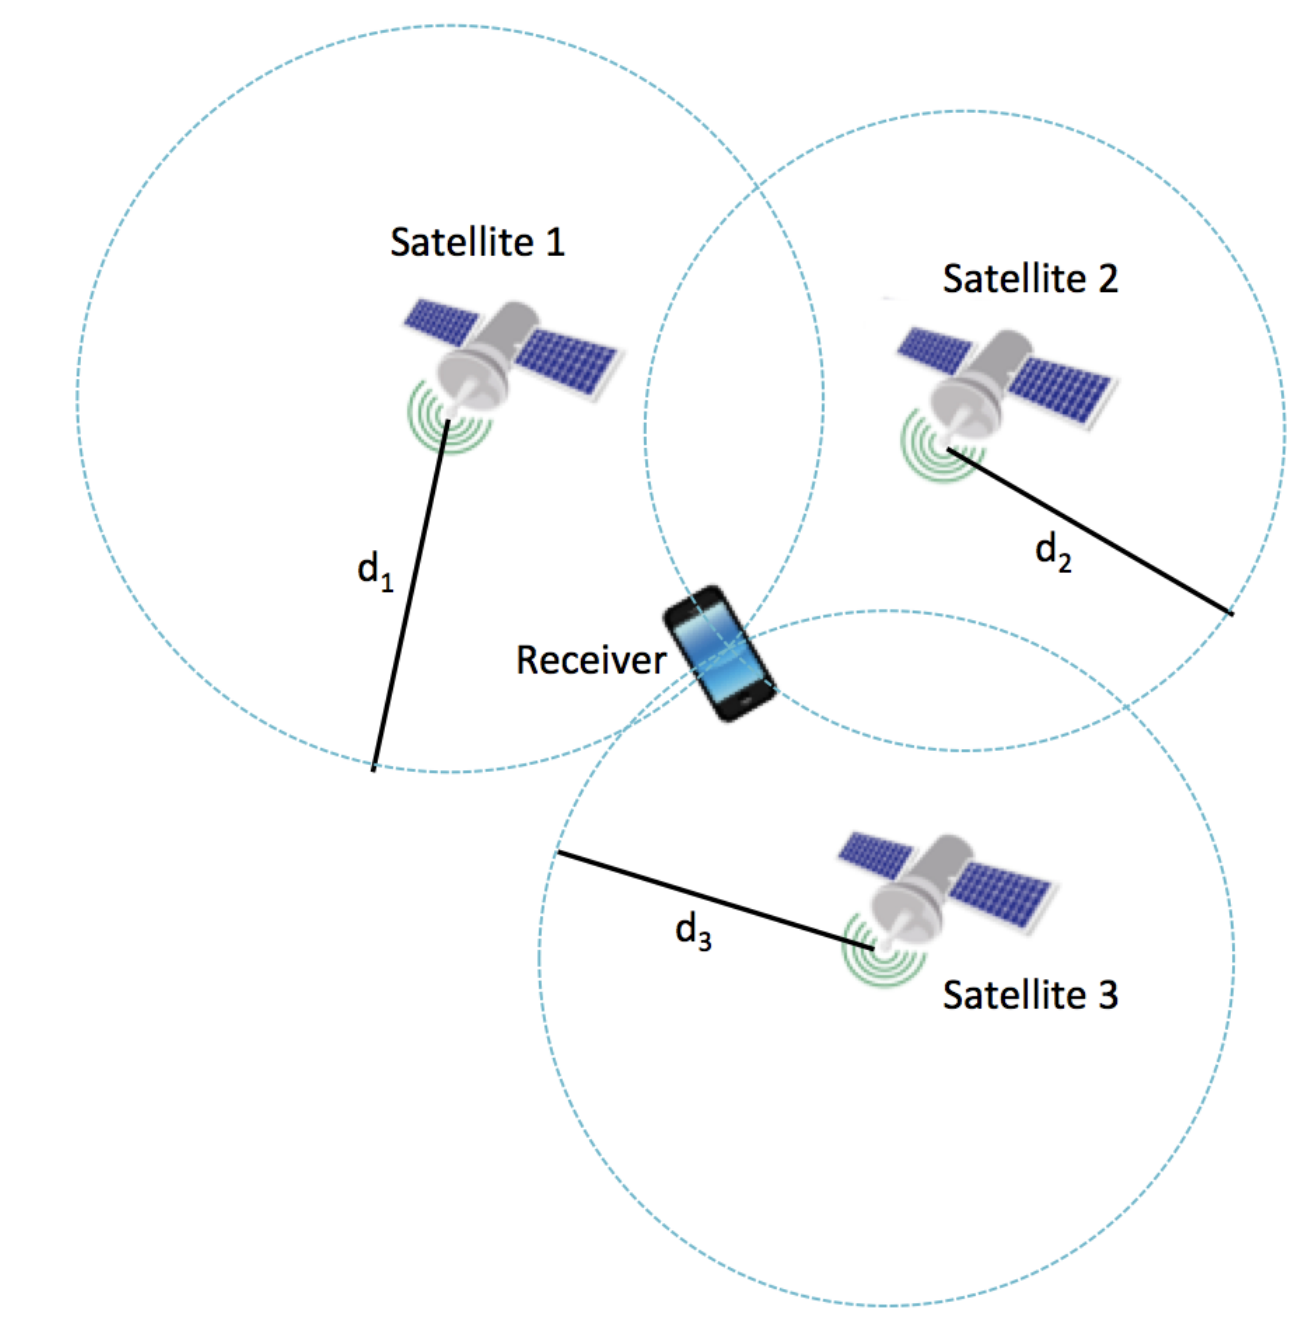
\includegraphics[scale=0.3]{../trilateration-2.png}
    \end{figure}

    \answerbox{4cm}

    % Paul can you answer this one? Not sure what concept you're testing here. It is kinda summarizing the ideas above one more time?

    \item Now that we have figured out where we are, it is time for us to decode the message! Recall that what our phone receives is a linear combination of these transmitted signals:
    $$\vec{r} = \alpha_1 \vec{s}_1^{\ (\tau_1)} + \alpha_2 \vec{s}_2^{\ (\tau_2)} + \hdots + \alpha_m \vec{s}_m^{\ (\tau_m)}$$
    From the expression above, which of the following variables are we trying to solve for?
    \begin{itemize}
        \item The scaling (attenuating) constant $\alpha_i$
        \item The original signal sent by the satellite $\vec{s}_i$
        \item The delay in the transmission of the signal $\tau_i$
    \end{itemize}

    \answerbox{3cm}

    \sol {
    \begin{itemize}
        \item The scaling (attenuating) constant $\alpha_i:$ These are \textbf{unknown} variables that we need to solve for since we receive one signal $\vec{r}$ that is a linear combination of the satellite signals and $\alpha_i$ are the weights of this linear combination.
        \item The original signal sent by the satellite $\vec{s}_i$ Remember that these are \textbf{known} variables that we as the engineer have programmed, hopefully using Gold Codes. No need to solve for these!
        \item The delay in the transmission of the signal $\tau_i$ While these were initially \textbf{unknown} variables, we solved for these in the second part using cross-correlation, so need to solve for these either!
    \end{itemize}
    }

    \item To solve for the unknown variables from the previous part, we can use the \textbf{least squares} method. How can we reformulate the given expression and information above as a \textbf{least squares} problem? In other words, if we are to rewrite the problem in the form:
    $$A\vec{v} \approx \vec{b},$$
    what would $A$, $\vec{v}$, and $\vec{b}$ be equal to respectively?
    
    \answerbox{4cm}

    \sol {
        The model for the received signal accounting for random noise $\vec{n}$ is:
        \[ \vec{r} = \alpha_1 \vec{s}_1^{\ (\tau_1)} + \alpha_2 \vec{s}_2^{\ (\tau_2)} + \hdots + \alpha_m \vec{s}_m^{\ (\tau_m)} + \vec{n} \]
        We can write this as the following matrix-vector equation:
        \[ 
        \vec{r} = 
        \begin{bmatrix} 
        | & | & | \\
        \vec{s}_1^{\ (\tau_1)} & \cdots & \vec{s}_m^{\ (\tau_m)} \\
        | & | & |
        \end{bmatrix}
        \begin{bmatrix} \alpha_{1} \\ \vdots \\ \alpha_{m} \end{bmatrix} + \vec{n}
        \]
        This can be formulated as a Least Squares problem with 
        $A = \begin{bmatrix} 
        | & | & | \\
        \vec{s}_1^{\ (\tau_1)} & \cdots & \vec{s}_m^{\ (\tau_m)} \\
        | & | & |
        \end{bmatrix},$ $\vec{v} = \begin{bmatrix} \alpha_{1} \\ \vdots \\ \alpha_{m} \end{bmatrix},$ and $\vec{b} = \vec{r}.$
        Note that $\vec{b}$ will not be in the column span of $A$ due to the noise, so we cannot solve this matrix-vector equation using Gaussian-Elimination. 
        We also cannot use matrix inversion, since we have made no assumptions of $A$ being square. 
    }

    \item What is the solution using the \textbf{least squares} method?
    
    \answerbox{3cm}

    \sol {
        The least-squares solution will be $\vec{\widetilde{v}} = (A^{T}A)^{-1} A^{T} \vec{b}.$
    }

    \item Does there exist a case where least squares would not work? Write down a sufficient condition where we have to resort to some other techniques to recover the original message.

    \note {
        The null-space proof was shown in lecture, but if students ask about it, you may want to go over it one more time.
        Take a look at lecture, or look up the proof in case they ask for it.
    }

    \sol {
        Least-Squares will fail when $A^{T}A$ is not an invertible matrix. 
        It can in fact be shown that $\text{Nul}(A) = \text{Nul}(A^{T} A)$ meaning the two subspaces will have the same dimensions.
        If $A$ is a $p \times m$ matrix, then $A^{T}A$ is a $m \times m$ matrix. 
        By the Rank-Nullity Theorem, $\text{dim Col} \ A^{T}A + \text{dim Nul} \ A^{T}A = m$ so we want $\text{dim Nul} \ A^{T} A$ to be zero for $A^{T}A$ to be invertible. Therefore, since $\text{dim Col} \ A + \text{dim Nul} \ A = p,$ and $\text{Nul} A = \text{Nul} \ A^{T} A,$ it must be that $\text{dim Col} \ A = p.$
        We conclude by saying that the matrix $A$ must be full-rank in order for Least-Squares to have a unique solution.
    }

    \answerbox{3cm}

    \item Now let's consider the case in which we have a large number of satellites or $(m >> n).$ Why can we no longer use Least-Squares anymore?

    \sol {
        If $m >> n,$ then the $A$ matrix will have more columns than rows, and will no longer be full rank since it will have linearly dependent columns.
        Therefore the matrix $A$ can only be at more rank $p$ meaning $A^{T}A$ will also only have at most rank $p < m$ meaning it will not be invertible.
    }

    \item We are now going to solve this problem using Orthogonal Matching Pursuit (OMP) instead of least squares, what is one assumption made by this technique?

    \note {
        If students ask about what to do when the sparsity assumption isn't made, tell them that it is out of scope for 16A, but they will learn how to handle this case in 16B.
    }

    \sol {
        In Orthogonal Matching Pursuit, we make the crucial assumption that the vector $\vec{v}$ is sparse. This means that most of the satellites will not be transmitting and most of the $\alpha$ coefficients will be zero. For example, if we have a total of $10,000$ satellites in space, then we make the assumption that only a small number, $(ex: 50)$ are transmitting a message. This is why we use a greedy, iterative algorithm to solve for the messages.
    }

    \answerbox{2cm}

    \item Describe what the stopping conditions for OMP are. In other words, how do we know when to stop running the OMP algorithm?

    \sol {
        In each step of OMP, we try to explain the data using our selected satellites $\vec{s}_{i}$ with the message $\alpha_{i}.$ 
        We then create an estimate $\vec{\widetilde{r}} = \sum\limits_{l = 1}^{k} \alpha_{l} \vec{s}_{l}^{\ (\tau_{l})}$ using the information we have. 
        The stopping condition of OMP will be when the residual $\vec{e} = \vec{r} - \vec{\widetilde{r}}$ is smaller than some threshold for us to say that we have explained the received signal $\vec{r}$ to the best of our ability.
    }

    \answerbox{2cm}

\end{enumerate}